\chapter{Fundamentos teóricos}
\label{chap:fundamentos-teoricos}
\vspace{0.5cm}



\lettrine{E}{n} este capítulo se introducen los fundamentos teóricos sobre los que se realizará el trabajo, en concreto acerca del ROBOBO! Framework, un framework de desarrollo creado específicamente para el ROBOBO.
%Este capítulo debería pasar a ser "Fundamentos teóricos o Conceptos previos" y debería incluir una descripción del ROBOBO Framework, qué usa (Android, ROS, etc)



\section{ROBOBO! Framework}
\label{sec:robobo-framework}

\begin{figure}
	\centering
	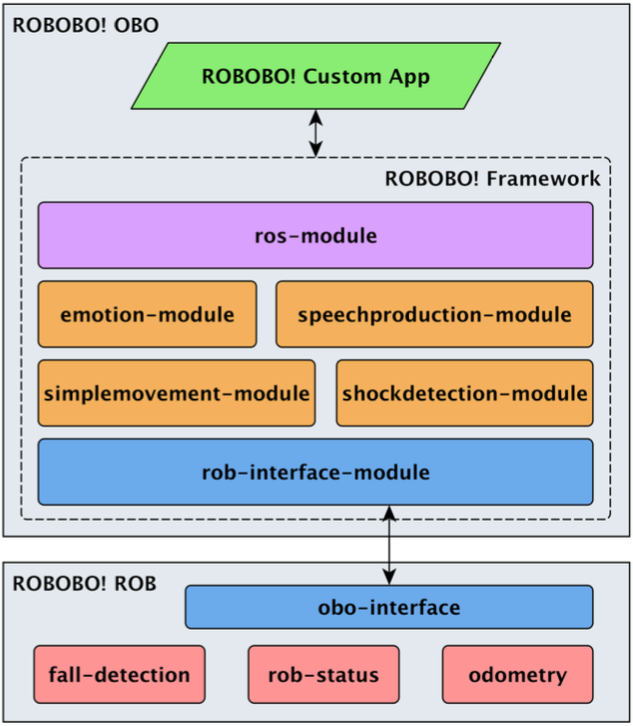
\includegraphics[width=0.6\linewidth]{imagenes/robobo_framework.png}
	\caption{Estructura de ROBOBO! framework dentro del entorno ROBOBO}
	\label{fig:robobo_framework_estructure}
\end{figure}
El ROBOBO! Framework es el marco de trabajo empleado para desarrollar el software para el ROBOBO y cuyas funcionalidades se expandirán mediante los módulos de interacción que se desarrollarán en este trabajo. 
El framework está enfocado al desarrollo de aplicaciones Android, sistema operativo del que se hablará en la sección \ref{subsec:android}, mediante el lenguaje de programación Java.
 
En la figura \ref{fig:robobo_framework_estructure} se puede ver como se estructura el sistema ROBOBO y cual es el rol del framework dentro del mismo.

La \textit{ROBOBO! Custom App}, de la figura, representa la aplicación final que el usuario instalará en su teléfono móvil y está construida sobre el framework, utilizando los diferentes módulos que este ofrece.

Dentro del framework se pueden encontrar diferentes módulos que proporcionan funcionalidades para el desarrollo de aplicaciones. Dos de ellos resultan especialmente importantes:

\paragraph*{ros-module:\\}
	 El \textit{ros-module}, proporciona una interfaz para pasar de acciones nativas del ROBOBO a conceptos propios de ROS, servicios o temas. Este modulo da acceso desde ROS a: 
	\begin{itemize}
		\item Las funcionalidades del ROB
		\item Los módulos del ROBOBO
		\item La cámara del dispositivo
		\item Los datos de los sensores del Smartphone
	\end{itemize} 
	Permite desarrollar tanto aplicaciones remotas, que no están alojadas en el smartphone pero  hacen uso de los servicios o temas ejecutándose en el ROBOBO, como aplicaciones ROS nativas.
	
Más adelante, en la sección \ref{subsec:ros}, se hablará con mas detalle de ROS .

\paragraph*{rob-interface-module:\\}
Este modulo nos permite obtener la interfaz de control de bajo nivel del robot, la clase \textit{IRob}(figura \ref{fig:irob}) , mediante el uso de esta interfaz se puede:

Recibir mensajes periódicos del estado del ROB:
\begin{itemize}
	\item Datos de los sensores de infrarrojos
	\item Información de detección de caídas
	\item Datos del movimiento de los motores
	\item Estado de la batería
\end{itemize}

Enviar comandos al ROB:
\begin{itemize}
	\item Movimiento de los motores
	\item Cambio de colores de los LEDs
	\item Modificación de la periodicidad de los mensajes de estado
	\item Cambiar el modo del ROB
\end{itemize}

\begin{figure}
	\centering
	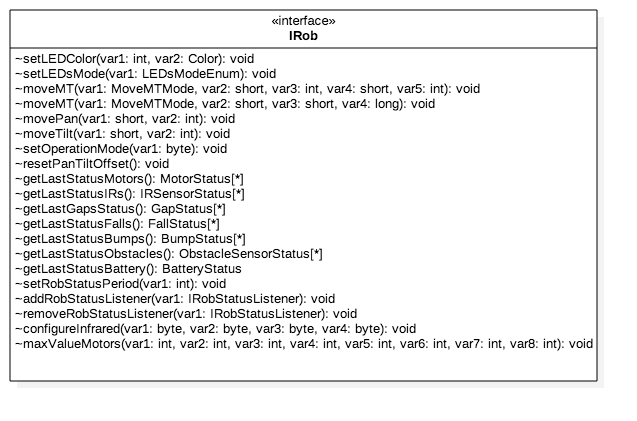
\includegraphics[width=0.9\linewidth]{imagenes/diagramas/IRob.png}
	\caption{Clase IRob}
	\label{fig:irob}
\end{figure}
Existen módulos para facilitar el uso del robot y evitar tener que usar la clase IRob, un ejemplo es el \textit{rob-movement-module}(figura \ref{fig:irob-movement}) que proporciona una interfaz de alto nivel para manejar los movimientos del robot.


\begin{figure}
	\centering
	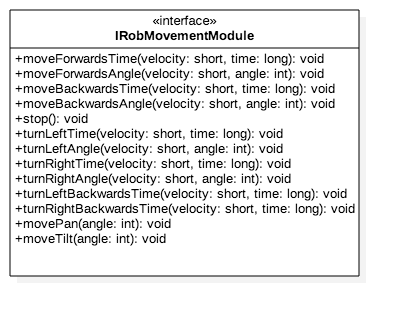
\includegraphics[width=0.9\linewidth]{imagenes/diagramas/IRobMovementModule.png}
	\caption{Clase IRobMovementModule}
	\label{fig:irob-movement}
\end{figure}



{\color{red} No tengo muy claro como funciona la parte que va dentro del ROB}

En el ROB se encuentra la \textit{obo-interface}, cuya finalidad es mantener la comunicación con el smartphone, y una serie de módulos programados en el firmware de la plataforma como la odometría y la detección de caídas.
%El ROBOBO! Framework es el framework de desarrollo usado para desarrollar aplicaciones para el ROBOBO en terminales móviles Android. Está diseñado de manera modular, de forma que facilita la extensión del mismo con nuevos módulos. Está publicado con una licencia libre LGPL v3 en Bitbucket\cite{RoboboFramework}.
%Ofrece el módulo \textit{rob-interface-module}, que permite la comunicación entre la plataforma robotizada (denominada ROB, figura \ref{fig:robobo_2_0}) y el smartphone (denominado OBO en el sistema) mediante el protocolo Bluetooth. También proporciona el módulo \textit{ros-module} que sirve de interfaz entre el robot y ROS \cite{Ros}.

El ROBOBO! Framework sigue una filosofía modular, para ello proporciona una interfaz común, \textit{IModule}(figura \ref{fig:imodule}), para los módulos que permite al framework gestionar el arranque y la finalización de los mismos


\begin{figure}
	\centering
	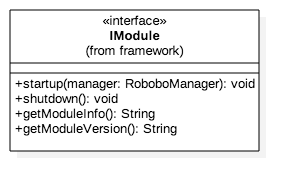
\includegraphics[width=0.7\linewidth]{imagenes/diagramas/IModule.png}
	\caption{Interfaz IModule}
	\label{fig:imodule}
\end{figure}
\subsection{Android}
\label{subsec:android}
%todo cambiar esto


Android es un sistema operativo de código abierto desarrollado por Google enfocado a dispositivos móviles. Actualmente es el sistema operativo más extendido en cuanto a terminales móviles, ocupando un 82.8\% de la cuota de mercado en el segundo cuarto de 2015 (IDC, Aug 2015) y contando la tienda de aplicaciones de la plataforma, la  Play Store, a Junio de 2016 con 2.2 millones de aplicaciones disponibles.
Dados estos datos de extensión y con la capacidad de cómputo y sensorización de los teléfonos se escogió este sistema como base para el ROBOBO.
Android está construido sobre un núcleo Linux sobre el cual corre el \textit{Android Runtime}(ART) o en versiones anteriores del sistema operativo la máquina virtual \textit{Dalvik}, siendo estos los entornos de ejecución de las propias aplicaciones Android.


\subsection{ROS}
\label{subsec:ros}
%todo cambiar esto
%\textbf{Sacado de la wikipedia a modo de placeholder}\\

El Sistema Operativo Robótico\cite{Ros} , por sus siglas en inglés ROS, es un framework libre de desarrollo de software para robots que provee los servicios que se podrían esperar de un sistema operativo, tales como la abstracción del hardware, la gestión de dispositivos a bajo nivel, implementación de funcionalidades comunes, paso de mensajes entre procesos y gestión de paquetes, sin embargo, ROS no es un sistema operativo y debe ejecutarse sobre un entorno Linux.
ROS esta organizado en forma de grafo en el cual los diferentes procesos procesan datos en red. En esta red podemos encontrar diferentes elementos:
\begin{itemize}
	\item Nodos:procesos que realizan una computación. Un sistema de control robótico suele contar con multitud de ellos que procesan datos en paralelo.
	\item Master: provee servicios de registro de nombres y consulta al resto del grafo computacional, funciona como punto de encuentro entre varios nodos.
	
	\item Servidor de parámetros: permite almacenar datos bajo un indice en una ubicación central, es parte del Master.
	\item Mensajes: Sistema de comunicación entre nodos, estructuras de datos formadas por tipos simples.
	\item Temas(topics): Semejante a un bus de datos, permite la generación de mensajes y la suscripción al mismo por parte de un nodo para recibirlos.
	\item Servicios: Mecanismo que permite a un nodo recibir peticiones y responderlas de manera concreta.
	\item Bolsas(bags): formato para almacenar y reproducir mensajes. Permite la reutilización de datos como los de sensorización para ser empleados posteriormente en desarrollo o pruebas.
\end{itemize}

ROS cuenta con una amplia comunidad a lo largo del mundo que contribuye de manera activa al proyecto. 
El repositorio de software de ROS contiene multitud de paquetes que proporcionan funcionalidades de forma simple, de manera que el programador pueda centrarse en el desarrollo del control de su robot sin tener que preocuparse de implementar los algoritmos y técnicas más comunes.

La funcionalidad de utilizar ROS en el ROBOBO esta provista por el módulo del ROBOBO! Framework \textit{ros-module} que  emplea la librería \textbf{rosjava} para este cometido.











 